% 导言区：格式定义
\documentclass[12pt,a4paper]{article} 
\usepackage{geometry} 
\geometry{left=2.5cm, right=2.5cm, top=2.5cm, bottom=2.5cm}
\usepackage{graphicx} 
\usepackage{float} 
\usepackage{booktabs} 
\usepackage{amsmath} 
\renewcommand{\baselinestretch}{1.15} 

% 强制所有段落首行缩进
\usepackage{indentfirst}
\setlength{\parindent}{2em} 

% 强制 section 和 subsection 标题全部居中且加粗
\usepackage{titlesec}
\titleformat{\section}[block]{\large\bfseries\filcenter}{}{0pt}{}
\titleformat{\subsection}[block]{\normalsize\bfseries\filcenter}{}{0pt}{}

% 文章主标题、作者、邮箱
\title{\textbf{\Large Regression Analysis: From Linear Optimization to Non-linear Kernel Methods}} 
\author{Your Name\\ 
Your\_Email@example.com} % 记得替换自己的名字和邮箱
\date{} 

\begin{document}
\maketitle 

\begin{abstract}
Regression analysis is a fundamental technique in statistical learning aimed at modeling the robust mapping from input features to continuous output values. In this report, we conduct a comprehensive comparative study on a 2-dimensional dataset. We initially evaluate three classic linear optimization algorithms: Ordinary Least Squares (OLS), Gradient Descent (GD), and Newton's Method. Observing significant underfitting due to the inherent non-linear nature of the data, we subsequently introduce Polynomial Regression and Radial Basis Function (RBF) Kernel Regression. The experimental results demonstrate that while linear methods share identical convergence in convex parameter spaces, basis function expansions and kernel tricks effectively capture local fluctuations, substantially improving both model accuracy and generalization capability.
\end{abstract}

\section*{Introduction}
The core challenge of regression lies in finding a hypothesis that not only fits the training data well but also generalizes effectively to unseen data. This involves delicately balancing model complexity to navigate the Bias-Variance Tradeoff. Simple models often suffer from high bias (underfitting), whereas overly complex models are prone to high variance (overfitting). 

In this study, we are provided with the \textit{Data4Regression} dataset, encompassing both training and testing sets. Initially, linear models are employed as the baseline due to their mathematical simplicity and interpretability. We analyze the convergence behaviors of three distinct optimization strategies. However, given that real-world data rarely strictly follow a straight line, linear models inevitably fail to capture complex data variances. To resolve this, we expand our hypothesis space by introducing non-linear basis functions. Specifically, we explore Polynomial Regression and Kernel Ridge Regression (utilizing a Gaussian RBF kernel). By systematically comparing their Mean Squared Errors (MSE) and $R^2$ scores, this report highlights the critical importance of model selection and feature mapping in the field of Pattern Recognition and Machine Learning (PRML).

\section*{Methodology}

\subsection*{M1: Linear Optimization Algorithms}
For a given dataset $\{x_i, y_i\}_{i=1}^N$, the objective of linear regression is to find the optimal weight vector $w$ that minimizes the Mean Squared Error (MSE) loss function $L(w) = \frac{1}{N} \|Xw - Y\|^2$. We investigate three approaches to solve this convex optimization problem:
\begin{itemize}
    \item \textbf{Ordinary Least Squares (OLS):} This method provides a direct, closed-form analytical solution by setting the gradient to zero. The optimal parameters are calculated as $w^* = (X^T X)^{-1} X^T Y$. It is highly efficient for low-dimensional datasets.
    \item \textbf{Gradient Descent (GD):} An iterative first-order optimization algorithm. The weights are updated step-by-step in the direction of the negative gradient: $w_{t+1} = w_t - \alpha \nabla L(w_t)$, where $\alpha$ is the learning rate and $\nabla L(w) = \frac{2}{N} X^T (Xw - Y)$.
    \item \textbf{Newton's Method:} A second-order numerical optimization technique utilizing the Hessian matrix $H = \frac{2}{N} X^T X$. The update rule is $w_{t+1} = w_t - H^{-1} \nabla L(w_t)$. Because the MSE loss function is a perfect quadratic bowl, Newton's method optimally converges to the global minimum in a single iteration.
\end{itemize}

\subsection*{M2: Polynomial Basis Expansion}
To overcome the underfitting of linear models, we map the 1D input $x$ into a higher-dimensional feature space using polynomial basis functions. The mapping is defined as $\phi(x) = [1, x, x^2, \dots, x^M]^T$, where $M$ is the polynomial degree. The model then becomes $y = w^T \phi(x)$. While increasing $M$ allows the model to capture more complex curves, an excessively large $M$ will lead to severe overfitting, amplifying data noise.

\subsection*{M3: Radial Basis Function (Kernel Regression)}
Kernel methods offer a powerful alternative for non-linear modeling without explicitly computing the transformed feature space. We employ Kernel Ridge Regression combined with a Gaussian Radial Basis Function (RBF) kernel, defined as:
\begin{equation}
    K(x, x') = \exp\left(-\gamma \|x - x'\|^2\right)
\end{equation}
where $\gamma$ acts as the bandwidth parameter controlling the smoothness of the function. The RBF kernel essentially maps the data into an infinite-dimensional Hilbert space, enabling the model to elegantly capture local periodic fluctuations and non-linear patterns.

\section*{Experimental Studies}
The experiments were conducted using Python. For the linear models, a bias term was appended. The Gradient Descent was executed with $\alpha = 0.01$ for 2000 epochs. 

As shown in Table \ref{tab:1}, OLS, GD, and Newton's Method all converged to the exact same global optimum, yielding a fitted line of approximately $y = 0.1089x - 0.6487$. Consequently, their training and testing MSEs are identically high (around $0.595$), and the $R^2$ score is extremely low ($0.0387$), providing empirical evidence of severe underfitting.

\begin{table}[H] 
    \centering 
    \caption{\textbf{Performance Comparison of Optimization and Regression Models}} 
    \begin{tabular}{lccc} 
        \toprule 
        \textbf{Model / Optimization} & \textbf{Training MSE} & \textbf{Test MSE} & \textbf{Test $R^2$} \\
        \midrule 
        Least Squares (Linear) & 0.6134 & 0.5950 & 0.0387 \\
        Gradient Descent (Linear) & 0.6134 & 0.5950 & 0.0387 \\
        Newton's Method (Linear) & 0.6134 & 0.5950 & 0.0387 \\
        \textbf{Polynomial (Degree=6)} & 0.4908 & 0.4497 & 0.2734 \\
        \textbf{RBF Kernel Reg} & \textbf{0.3644} & \textbf{0.3470} & \textbf{0.4393} \\
        \bottomrule 
    \end{tabular}
    \label{tab:1} 
\end{table}

Upon applying non-linear models, the performance significantly improved. The Polynomial Regression (Degree=6) reduced the test MSE to $0.4497$. However, the RBF Kernel Regression achieved the most outstanding results, dropping the test MSE to $0.3470$ and elevating the $R^2$ score to $0.4393$. 

Figure \ref{fig:1} visually contrasts these approaches. The red dashed line strictly illustrates the rigidity of the linear assumption. The blue curve (Polynomial) attempts to follow the data but exhibits slight instability at the boundaries. The green curve (RBF Kernel) successfully and smoothly traverses the dense data clusters, demonstrating a superior balance between model complexity and generalization.

\begin{figure}[H] 
    \centering 
    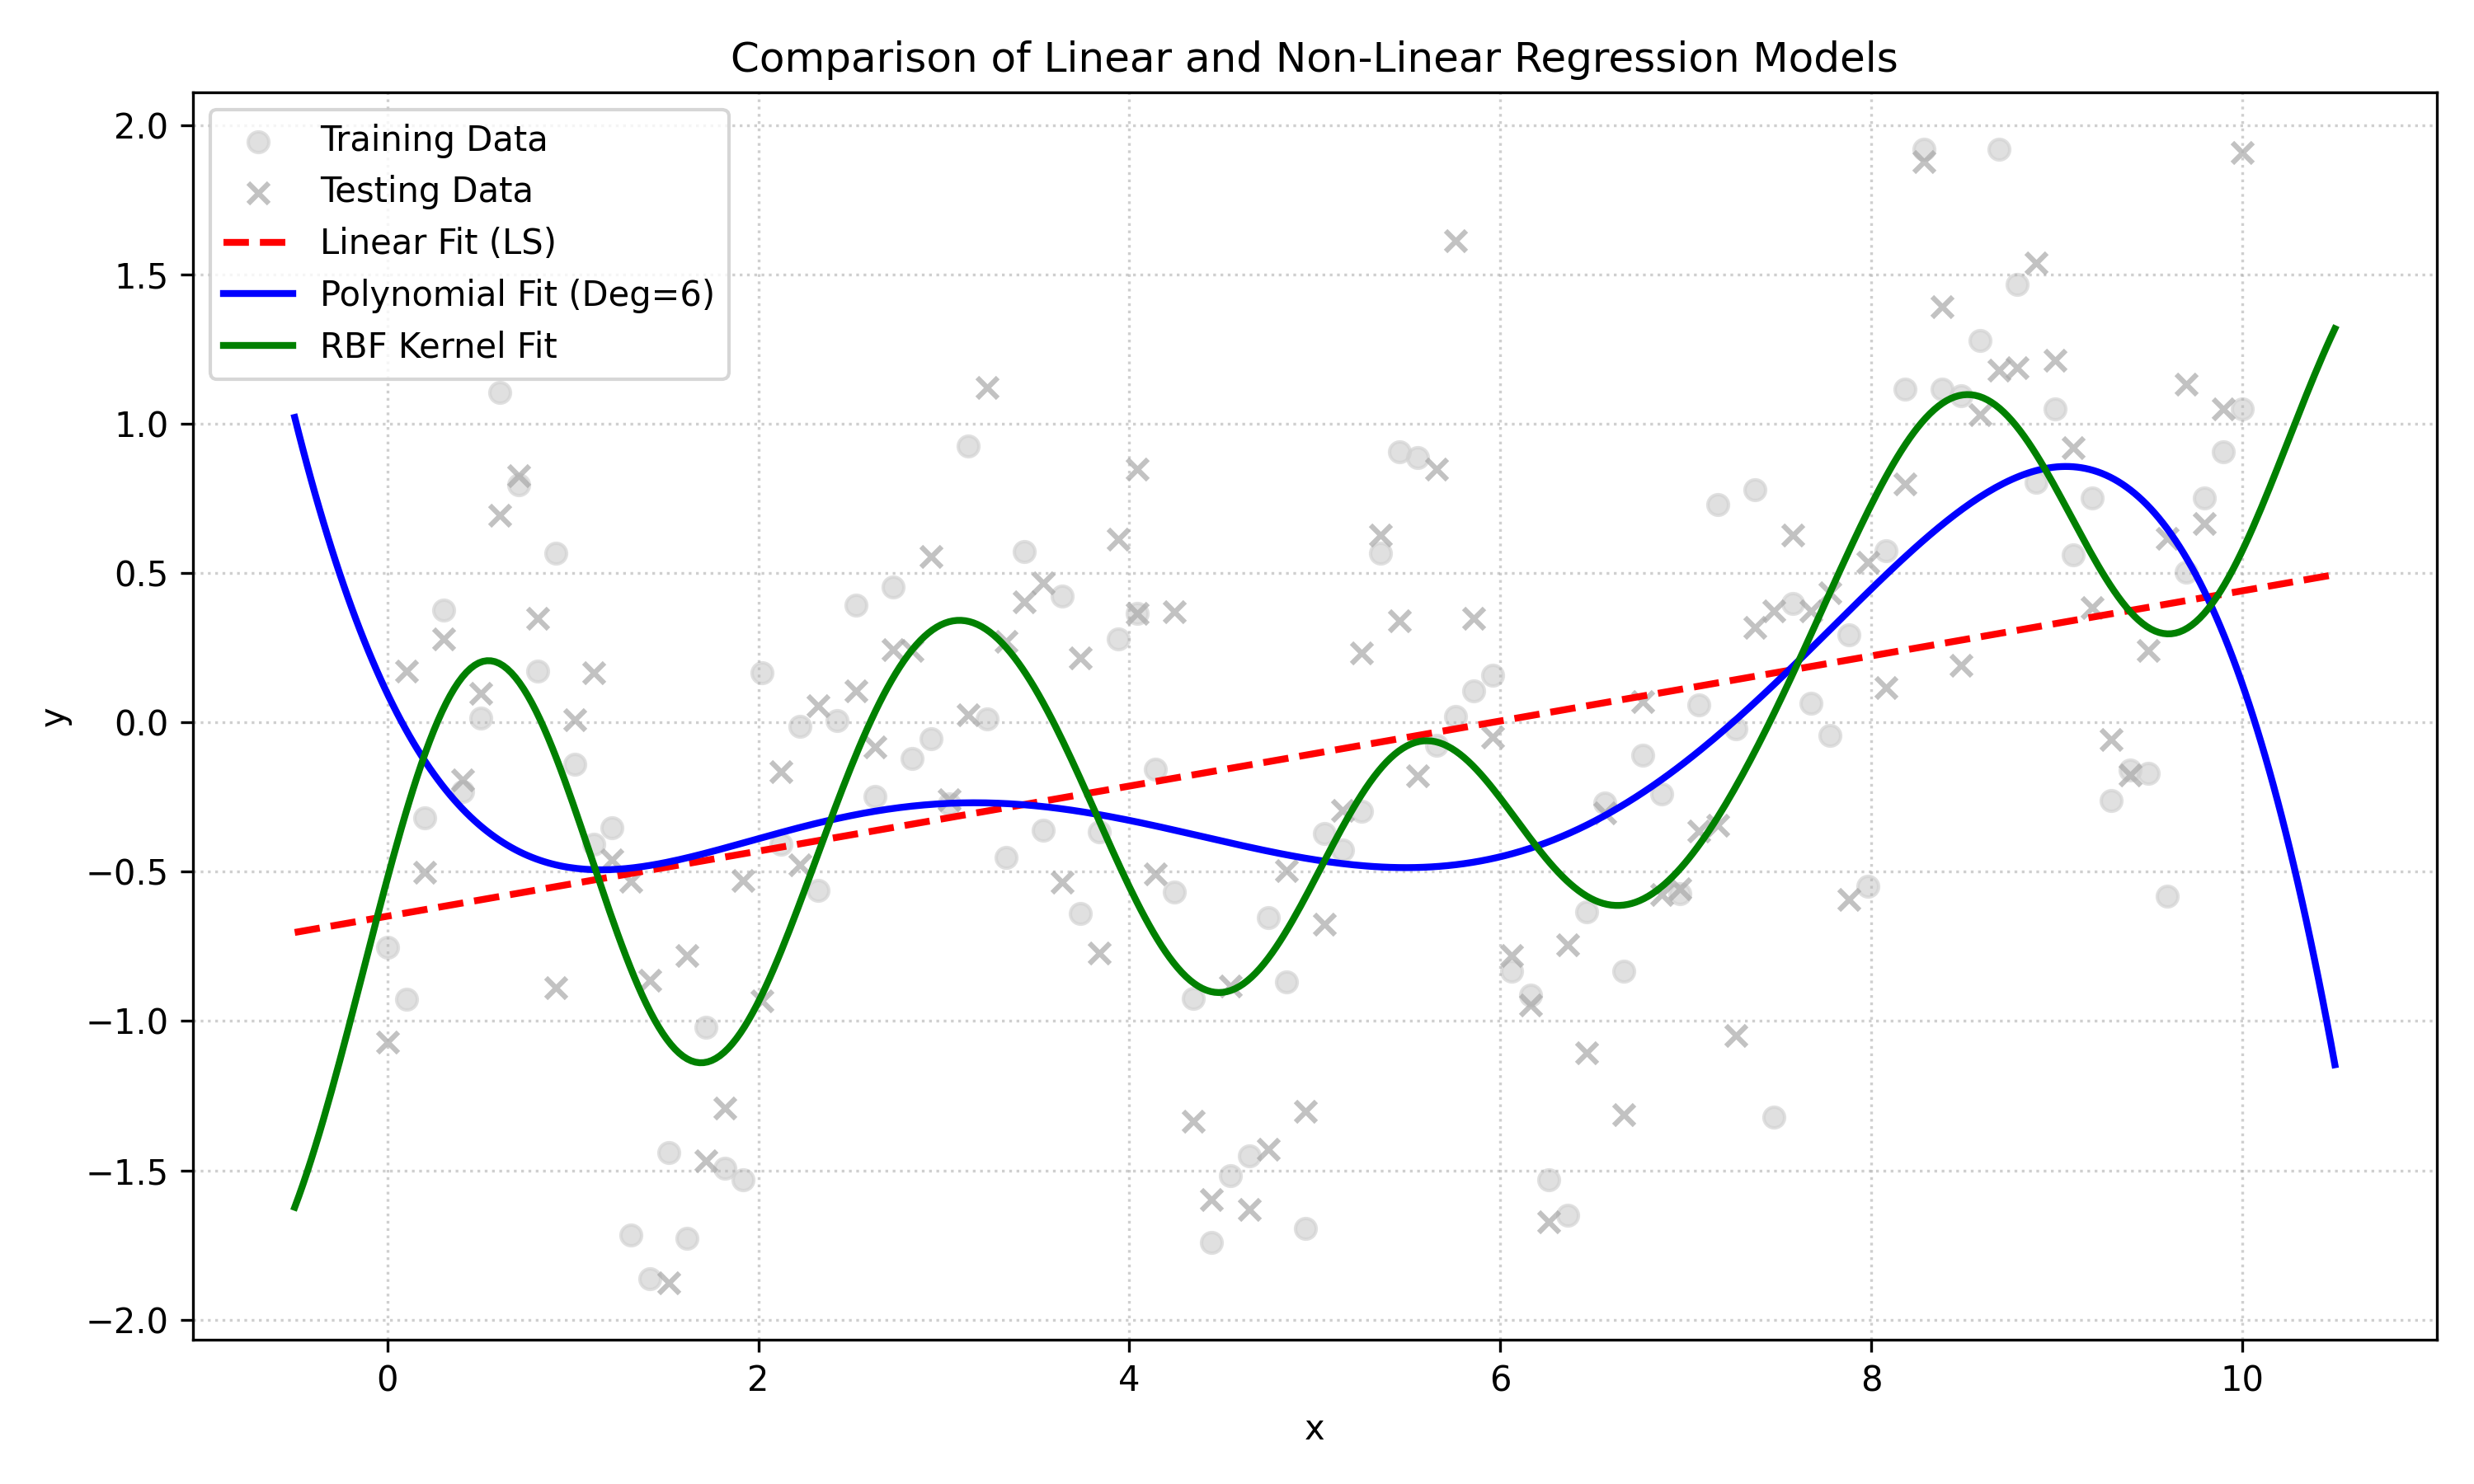
\includegraphics[width=0.9\textwidth]{fit_results.png}
    \caption{\textbf{Visual Comparison of Linear and Non-linear Regressions on the Dataset}}
    \label{fig:1}
\end{figure}

\section*{Conclusions}
This study systematically investigated the application of diverse regression models and optimization techniques. We conclude that while linear models (OLS, GD, Newton's Method) provide mathematically robust and efficient convergence, they are fundamentally inadequate for non-linear data distributions. By leveraging feature engineering and basis function expansions—specifically Polynomial mapping and RBF Kernel tricks—the model's capacity to fit complex curves is vastly enhanced. Ultimately, RBF Kernel Regression demonstrated the best predictive performance, underscoring the necessity of selecting models and hyperparameters that appropriately align with the intrinsic geometry of the data to maintain generalization.

\section*{References}
\begin{enumerate}
    \item[1] Bishop, C. M. (2006). \textit{Pattern Recognition and Machine Learning}. Springer.
    \item[2] Goodfellow, I., Bengio, Y., and Courville, A. (2016). \textit{Deep Learning}. MIT Press.
    \item[3] Hastie, T., Tibshirani, R., and Friedman, J. (2009). \textit{The Elements of Statistical Learning}. Springer.
\end{enumerate}

\end{document}